\documentclass[10pt,a4paper]{article}
\usepackage[left=2.00cm, right=2.00cm, bottom=2.00cm]{geometry}
\usepackage[latin1]{inputenc}
\usepackage{amsmath}
\usepackage{amsfonts}
\usepackage{amssymb}
\usepackage{graphicx}
\usepackage{tikz}

\title{Concept}
\author{Mikail Gedik}
\date{2020-05-07}
\begin{document}
	\maketitle
	\begin{center}
		Betreungsperson: Peter Holzer\\
		Revision 1
	\end{center}
	\tableofcontents
	\newpage
	
	\section{General}
	My thesis paper resolves around the efficient programming of (a few) fractals. Because of this, my thesis has two aspects, the mathematical one and the computer science. I am concentrating myself more on the latter, but that may change as i progress in my work.
	\section{IDEs and other programming tools}
	I have experience with the IntelliJ Idea, CLion Idea and Mathematica. I aim to use IntelliJ and CLion for development in Java and C++ respectively. Mathematica can be very use when searching and testing algorithms.
	\section{VCS \textit{(Version Control System)} - git}
	I want to introduce this section with one small memory I made during this year's presentation of the Maturaarbeiten. He had dedicated an entire page of his presentation to one short sentence: "Git saves lives".\\
	According to him, he would have had a lot of problems if it had not been for git. The possibility to roll back an older point of one's project, the option to test multiple solutions to a problem using branches and the fact that is widely supported on the most common platforms and IDEs.\\
	The rough concept, the concept and the thesis itself are all in the same repository and also tracked by git. I plan to upload my repository on Github or to my own server, so that I have backups in case of an emergency and others may take a peek at my code and give me tips.
	\section{Writing Tool: \LaTeX}
	Instead of using a WYSIWYG \textit{(What you see is what you get)} tool like Microsoft Word, I prefer using \LaTeX(compiled with MiKTeX and TeXstudio). In my opinion they are better for writing mathematical papers, as they provide an excellent output for formulas. Furthermore, I may add lots of images like plots and the like. Through the \textit{TikZ}-package, it is easily possible to create these. On top of that, the file size of documents containing plots created with this package is considerably smaller than documents using images. This simplifies the distribution of my thesis and guarantees me not to run into any file size restrictions of the school-email (15 Megabytes).
	\section{Content}
	\subsection{Mathematics}
	I plan to start with the most common fractal, the Mandelbrot set. After that one, I may try the Julia set, because of their similarity. Further fractals may be more complex to implement, as each has their own perfect optimization.\\
	I will have to find further material regarding the fractals.
	\subsection{Computer Science}
	The first prototype will be implemented in Java, following that there will be a C++ implementation. My project will be modularized in (at least) a front end and a back end. Because they are completely detached from each other, I may even be able program on in one language and the other in another.\\
	Instead of just making a new project and starting to program, I first plan to have a rough shape of what files/classes that will be used and in which order they will be implement. 
	\subsubsection{Structure}
	\begin{center}
		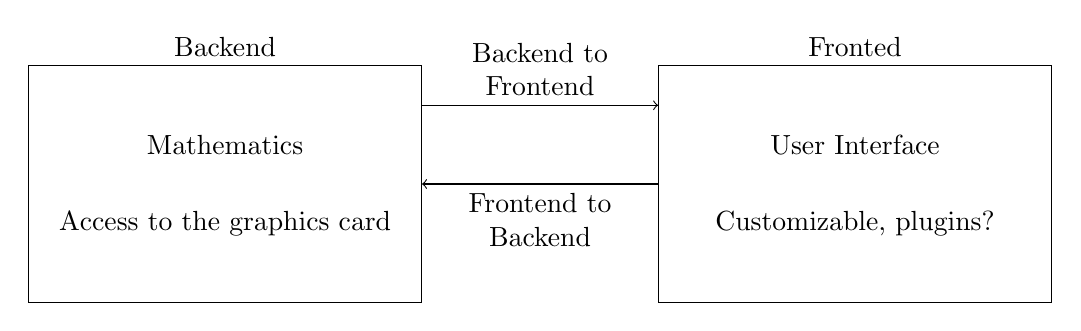
\begin{tikzpicture}
		\draw (0,0) rectangle (5,3);
		\draw (8,0) rectangle (13,3);
		\node[above] at (2.5,3) {Backend};
		\node[above] at (10.5,3) {Fronted};
		
		\node at (2.5,2) {Mathematics};
		\node at (2.5,1) {Access to the graphics card};
		
		\node at (10.5,2) {User Interface};
		\node at (10.5, 1) {Customizable, plugins?};
		
		\draw[->] (5,2.5) -- (8,2.5);
		\node[above, align = center] at (6.5, 2.5) {Backend to\\ Frontend};
		
		\draw[->] (8,1.5) -- (5,1.5);
		\node[below, align = center] at (6.5, 1.5) {Frontend to\\ Backend};
		\end{tikzpicture}
	\end{center}
	\section{Time Management}
	The deadline for the thesis is the 30 November 2020. My intention is to have a working prototype of my program which is able to run by the summer break. From then on, I will perform slighter adjustments and performance tweaks like making it platform independent or improving its user interface.
	\begin{table}[h]
		\centering
		\begin{tabular}{l|l}
			Date & Working status \\ \hline
			2020-05-10 & Started work on the thesis paper\\ \hline
			2020-05-31 & Defined structure of code and started working on it \\ \hline
			2020-06-28 & All sources found, thesis paper halfway finished \\ \hline
			2020-07-19 & Implemented all central aspects \\ \hline
			2020-08-09 & Finished first rough draft of thesis paper \\ \hline
			2020-09-06 & Added friendlier UI, performance optimizations \\ \hline
			2020-10-04 & Finished corrections of paper \\ \hline
			2020-11-01 & Posing print job \\ \hline
			2020-11-30 & Deadline \\
		\end{tabular}
	\end{table}
\end{document}